\documentclass[12pt,a4paper,bibliography=totocnumbered,listof=totocnumbered]{scrartcl}
\usepackage[ngerman]{babel}
\usepackage[utf8]{inputenc}
\usepackage{amsmath}
\usepackage{amsfonts}
\usepackage{amssymb}
\usepackage{graphicx}
\usepackage{fancyhdr}
\usepackage{tabularx}
\usepackage{geometry}
\usepackage{setspace}
\usepackage[right]{eurosym}
\usepackage[printonlyused]{acronym}
\usepackage{subfig}
\usepackage{floatflt}
\usepackage[usenames,dvipsnames]{color}
\usepackage{colortbl}
\usepackage{paralist}
\usepackage{array}
\usepackage{titlesec}
\usepackage{parskip}
\usepackage[right]{eurosym}
\usepackage{picins}
\usepackage[subfigure,titles]{tocloft}
\usepackage[pdfpagelabels=true]{hyperref}

\usepackage{listings}
\lstset{basicstyle=\footnotesize, captionpos=b, breaklines=true, showstringspaces=false, tabsize=2, frame=lines, numbers=left, numberstyle=\tiny, xleftmargin=2em, framexleftmargin=2em}
\makeatletter
\def\l@lstlisting#1#2{\@dottedtocline{1}{0em}{1em}{\hspace{1,5em} Lst. #1}{#2}}
\makeatother

\geometry{a4paper, top=27mm, left=30mm, right=25mm, bottom=35mm, headsep=10mm, footskip=12mm}

\hypersetup{unicode=false, pdftoolbar=true, pdfmenubar=true, pdffitwindow=false, pdfstartview={FitH},
	pdftitle={Bachelorarbeit},
	pdfauthor={Nils Lutz},
	pdfsubject={Bachelorarbeit},
	pdfcreator={\LaTeX\ with package \flqq hyperref\frqq},
	pdfproducer={pdfTeX \the\pdftexversion.\pdftexrevision},
	pdfkeywords={Bachelorarbeit},
	pdfnewwindow=true,
	colorlinks=true,linkcolor=black,citecolor=black,filecolor=magenta,urlcolor=black}
\pdfinfo{/CreationDate (D:20141022170944)}

\begin{document}

\titlespacing{\section}{0pt}{12pt plus 4pt minus 2pt}{-6pt plus 2pt minus 2pt}

% Kopf- und Fusszeile
\renewcommand{\sectionmark}[1]{\markright{#1}}
\renewcommand{\leftmark}{\rightmark}
\pagestyle{fancy}
\lhead{}
\chead{}
\rhead{\thesection\space\contentsname}
\lfoot{Analyse und Realisierung einer prototypischen\newline Portal Applikation im SAP Kontext/Umfeld}
\cfoot{}
\rfoot{\ \linebreak Seite \thepage}
\renewcommand{\headrulewidth}{0.4pt}
\renewcommand{\footrulewidth}{0.4pt}

% Vorspann
\renewcommand{\thesection}{\Roman{section}}
\renewcommand{\theHsection}{\Roman{section}}
\pagenumbering{Roman}

% ----------------------------------------------------------------------------------------------------------
% Titelseite
% ----------------------------------------------------------------------------------------------------------
\thispagestyle{empty}
\begin{center}
	
\includegraphics[scale=0.7]{images/fh_whv_big.jpg}\\
	\vspace*{2cm}
	\Large
	\textbf{Jade Hochschule}\\
	\textbf{Management, Information \& Technologie}\\
	\textbf{Wirtschaftsinformatik}\\
	\vspace*{2cm}
	\Huge
	\textbf{Bachelorarbeit}\\
	\vspace*{0.5cm}
	\large
	über das Thema\\
	\vspace*{1cm}
	\textbf{Analyse und Realisierung einer prototypischen Portal Applikation im SAP Kontext/Umfeld}\\
	\vspace*{2cm}
	
	\vfill
	\normalsize
	\newcolumntype{x}[1]{>{\raggedleft\arraybackslash\hspace{0pt}}p{#1}}
	\begin{tabular}{x{6cm}p{7.5cm}}
		\rule{0mm}{5ex}\textbf{Autor:} & Nils Lutz\newline info@nilslutz.de \\ 
		\rule{0mm}{5ex}\textbf{Erstprüfer:} & Prof. Dr.-Ing. Hergen Pargmann \\ 
		\textbf{Zweitprüfer:} & Prof. Dr. Harald Schallner \\ 
		\rule{0mm}{5ex}\textbf{Abgabedatum:} & 25.01.2015  \\ 
	\end{tabular} 
\end{center}
\pagebreak

% ----------------------------------------------------------------------------------------------------------
% Abstract
% ----------------------------------------------------------------------------------------------------------
\setcounter{page}{1}
\onehalfspacing
\titlespacing{\section}{0pt}{12pt plus 4pt minus 2pt}{2pt plus 2pt minus 2pt}
\rhead{KURZFASSUNG}
\section{Kurzfassung}
Lorem ipsum dolor sit amet, consetetur sadipscing elitr, sed diam nonumy eirmod tempor invidunt ut labore et dolore magna aliquyam erat, sed diam voluptua. At vero eos et accusam et justo duo dolores et ea rebum. Stet clita kasd gubergren, no sea takimata sanctus est Lorem ipsum dolor sit amet. Lorem ipsum dolor sit amet, consetetur sadipscing elitr, sed diam nonumy eirmod tempor invidunt ut labore et dolore magna aliquyam erat, sed diam voluptua. At vero eos et accusam et justo duo dolores et ea rebum. Stet clita kasd gubergren, no sea takimata sanctus est Lorem ipsum dolor sit amet. 

\vspace{-1,2em}
\titlespacing{\section}{0pt}{12pt plus 4pt minus 2pt}{-6pt plus 2pt minus 2pt}
\section*{Abstract}
Das ganze auf Englisch.
\pagebreak

% ----------------------------------------------------------------------------------------------------------
% Verzeichnisse
% ----------------------------------------------------------------------------------------------------------
% TODO Typ vor Nummer
\renewcommand{\cfttabpresnum}{Tab. }
\renewcommand{\cftfigpresnum}{Abb. }
\settowidth{\cfttabnumwidth}{Abb. 10\quad}
\settowidth{\cftfignumwidth}{Abb. 10\quad}

\titlespacing{\section}{0pt}{12pt plus 4pt minus 2pt}{2pt plus 2pt minus 2pt}
\singlespacing
\rhead{INHALTSVERZEICHNIS}
\renewcommand{\contentsname}{II Inhaltsverzeichnis}
\phantomsection
\addcontentsline{toc}{section}{\texorpdfstring{II \hspace{0.35em}Inhaltsverzeichnis}{Inhaltsverzeichnis}}
\addtocounter{section}{1}
\tableofcontents
\pagebreak
\rhead{VERZEICHNISSE}
\listoffigures
\pagebreak
\listoftables
%\pagebreak
\renewcommand{\lstlistlistingname}{Listing-Verzeichnis}
{\labelsep2cm\lstlistoflistings}
\pagebreak

% ----------------------------------------------------------------------------------------------------------
% Abkürzungen
% ----------------------------------------------------------------------------------------------------------
\section{Abkürzungsverzeichnis}
\begin{acronym}[OSGi] % längste Abkürzung steht in eckigen Klammern
	\setlength{\itemsep}{-\parsep} % geringerer Zeilenabstand
	\acro{OSGi}{Open Service Gateway initiative}
	\acro{JSP}{Java Server Pages}
	\acro{BSP}{Business Server Pages}
	\acro{SPP}{Spare Parts Planning}
\end{acronym}
\newpage

% ----------------------------------------------------------------------------------------------------------
% Inhalt
% ----------------------------------------------------------------------------------------------------------
% Abstände Überschrift
\titlespacing{\section}{0pt}{12pt plus 4pt minus 2pt}{-6pt plus 2pt minus 2pt}
\titlespacing{\subsection}{0pt}{12pt plus 4pt minus 2pt}{-6pt plus 2pt minus 2pt}
\titlespacing{\subsubsection}{0pt}{12pt plus 4pt minus 2pt}{-6pt plus 2pt minus 2pt}

% Kopfzeile
\renewcommand{\sectionmark}[1]{\markright{#1}}
\renewcommand{\subsectionmark}[1]{}
\renewcommand{\subsubsectionmark}[1]{}
\lhead{Kapitel \thesection}
\rhead{\rightmark}

\onehalfspacing
\renewcommand{\thesection}{\arabic{section}}
\renewcommand{\theHsection}{\arabic{section}}
\setcounter{section}{0}
\pagenumbering{arabic}
\setcounter{page}{1}

% ----------------------------------------------------------------------------------------------------------
% Einleitung
% ----------------------------------------------------------------------------------------------------------
\section{Einleitung}
\subsection{Motivation}
// wieso weshalb warum wo\\
// Beschreibung abatAG\\
// Enstehung des Projekts\\

\subsection{Problemstellung}
// aktuelle situationsbeschreibung\\
// was soll besser laufen\\

\pagebreak
\subsection{Zielsetzung}
// Das Produkt - Template Programmierung für SAP Frontends mit SAP UI5

\subsection{Struktur}
// der weg über die software ergonomie und ihre wichtigkeit, gezeigt über die Marktanalyse, hin zur praktischen Umsetzung durch Grundlagen und Beschreibung des Lösungsweges\\

\pagebreak
% ----------------------------------------------------------------------------------------------------------
% Kapitel
% ----------------------------------------------------------------------------------------------------------
\section{Software Ergonomie}
// Beleg für die Wichtigkeit von Software Ergonomie\\
// Kurze Übersicht über das Themenfeld Software Ergonomie\\
// Wichtigsten Aspekte nennen und näher erläutern\\

\subsection{Definition}
\subsubsection{Kognitionspsychologie}
// Modellierung und Simulation von menschlichen Denk- und Wahrnehmungsprozessen\\

\subsubsection{Arbeitsphysiologie, Industrieanthropologie}
// Beschäftigung mit grundlegenden menschlichen Fähigkeiten zur Informationsaufnahme und Informationsverarbeitung\\

\subsubsection{Arbeitspsychologie}
// Untersuchung der Wechselbeziehungen zwischen Arbeit, deren Schnittstellen und psychischen Faktoren (unter anderem Arbeitszufriedenheit und -unlust)\\

\subsection{DIN EN ISO 9241}
// DIN Norm zur Software Ergonomie\\
// Die 7 Grundsätze der Dialoggestaltung:
\begin{compactitem}
	\item Aufgabenangemessenheit
	\item Selbstbeschreibungsfähigkeit
	\item Erwartungskonformität
	\item Fehlertoleranz
	\item Steuerbarkeit
	\item Individualisierbarkeit
	\item Lernförderlichkeit
\end{compactitem}
\paragraph{DIN EN ISO 14915}
$\;$ \\
// Erweiterung der ISO 9241\\

\subsection{Wirtschaftlicher Faktor}
// Kosteneinsparungspotenzial finden und begründen\\

\subsection{Analyse Methoden}
\subsubsection{Eye Tracking}
// Funktionsweise und Ergebnis\\

\subsubsection{Mouse Clicking}
// Funktionsweise und Ergebnis\\

\subsection{SAP Technologien in Bezug auf Software Ergonomie}
\subsubsection{Business Server Pages}
// \ac{BSP} ist old school Technik\\
// geklaut von \ac{JSP}\\

\subsubsection{Web Dynpro for ABAP}
// Aktuelle Technik\\
// ABAP Code generiert HTML\\
// statischer und dynamischer Teil\\

\subsubsection{SAP Fiori / SAP UI5 / SAP Screen Personas}
// cutting edge\\
// aktuelle SAP UI Strategie\\
// SAP Präsi Chart Fiori/SP renew, etc. pp\\
// SAP Fiori einerseits Name des Themes/Guideline\\
// andererseits Bündel der gängigsten TAs/GPs als fertige\\
// Mobile First/Responsive Design Applikationen\\
// SAP UI5 - SAPs Framework zur Entwicklung von eigenen Applikationen im Fiori Style\\
// Nicht zu tief auf JS, HTML etc eingehen, dass kommt im nächsten Kapitel\\
// SAP SP - Zusätzliche Schicht um Standard Dynpro zu Personalisieren und so\\

\pagebreak
% ----------------------------------------------------------------------------------------------------------
% Kapitel
% ----------------------------------------------------------------------------------------------------------
\section{Technologien}
Lorem ipsum dolor sit amet.
%\subsection{Marktanalyse}
%\subsubsection{Nicht-SAP Lösung}
%// Oracle oder andere ERP Anbieter\\
%// jedoch müssen auch die Anforderungen von Claas abgedeckt sein\\
%
%\subsubsection{SAP Standard Lösung}
%// kann der SAP Standard das Abbilden was Claas haben will\\

\subsection{HTML5 und CSS3}
// Entstehung - Von Dez '97 bis Okt '14\\
// Abbildung \ref{fig:html5specs}\\
	\vspace{1em}
	\begin{minipage}{\linewidth}
		\centering
		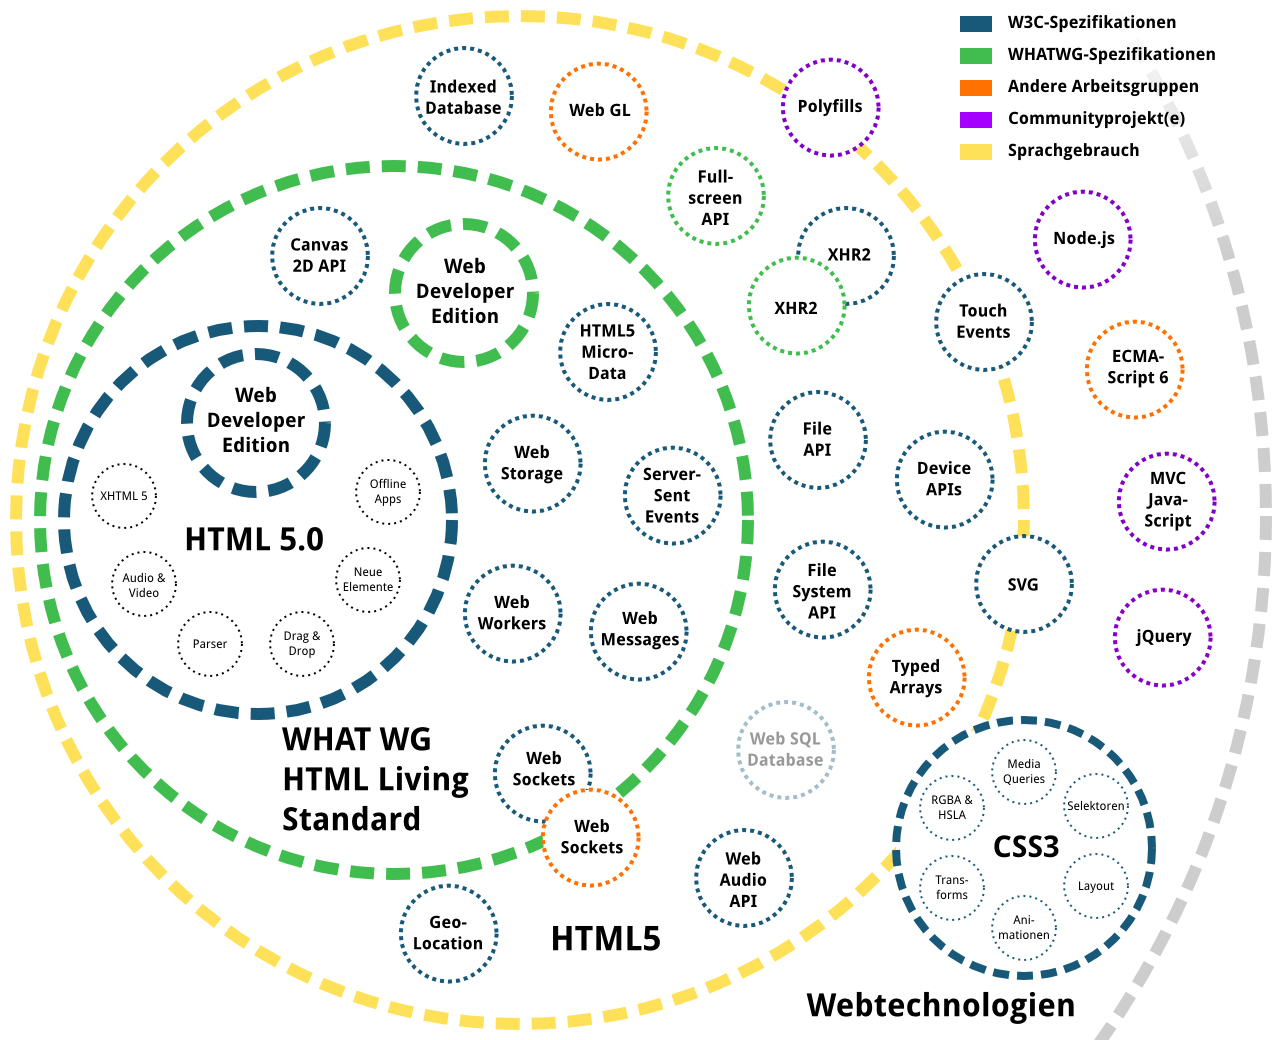
\includegraphics[width=1\linewidth]{images/html5_specs.png}
		\captionof{figure}[HTML5 Spezifikation Übersicht]{HTML5 Spezifikation Übersicht\footnotemark }
		\label{fig:html5specs}
	\end{minipage}
	\footnotetext{Quelle: \url{https://github.com/SirPepe/SpecGraph/blob/master/graph_w.png}}
	
// Ziele - Kompatibilität, Verwendbarkeit, Sicherheit, Konsistenz, Vereinfachung, Universalität, Barrierefreiheit\\
// Aufbau - Syntax, Start Tag, End Tag, Attributes\\
// Listing \ref{lst:html5basicdoc}
	\vspace{1em}
	\begin{lstlisting}[caption=HTML5 Basis Dokument, label=lst:html5basicdoc]
<!DOCTYPE html>
<html>
 <head>
  <title>Beispiel Seite</title>
 </head>
 <body>
  <h1>Beispiel Seite</h1>
  <p>Dies ist ein <a href="demo.html">einfaches</a> Beispiel.</p>
  <!-- dies ist ein Kommentar -->
 </body>
</html>
	\end{lstlisting}

// Wichtige neue Sprachelemente - Microdata (meta tags), 2D Canvas (canvas tag), Media (audio/video tags), Struktur (section, article, nav, aside, header, footer), Formular (input, ...), geänderte Elemente (b, i, hr, small, ...)\\

// CSS3\\
// Allgemeiner Aufbau - Gestaltungssprache, Kern Element des WWW, Darstellung und Inhalt getrennt, Unterschiedliche Optik je nach Ausgabe Gerät\\
// Syntax - Selektoren, Eigenschaften, Werte, Pseudoklassen\\
// Listing \ref{lst:css3syntax}
	\vspace{1em}
	\begin{lstlisting}[caption=CSS3 Syntax Beispiel, label=lst:css3syntax]
Selektor [, Selektor2, ...]
  {
    Eigenschaft-1: Wert-1;
    ...
    Eigenschaft-N: Wert-N[;]
  }
  /* Kommentar - In eckigen Klammern stehen optionale Angaben */
	\end{lstlisting}

// CSS-Box-Modell - margin, border, padding\\
// Abbildung \ref{fig:cssboxmodell}\\
	\vspace{1em}
	\begin{minipage}{\linewidth}
		\centering
		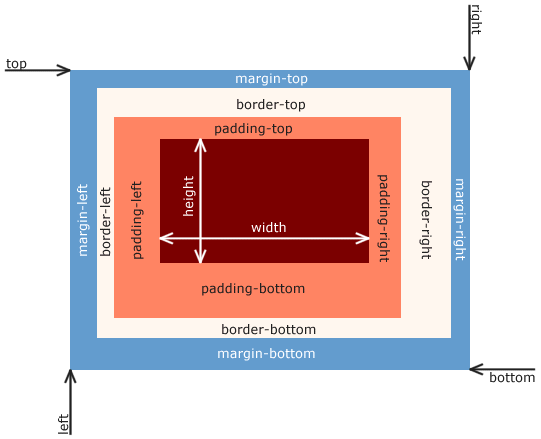
\includegraphics[width=0.7\linewidth]{images/css_boxmodell.png}
		\captionof{figure}[CSS-Boxmodell]{CSS-Boxmodell\footnotemark }
		\label{fig:cssboxmodell}
	\end{minipage}
	\footnotetext{Quelle: \url{http://commons.wikimedia.org/wiki/File:Boxmodell-detail.png}}
	
// Medienspezifische Stylesheets (@media print, screen, ...)\\
// Listing \ref{lst:css3media}
	\vspace{1em}
	\begin{lstlisting}[caption=CSS3 medienspezifisches Stylesheet, label=lst:css3media]
@media print {
	body {
		color: black;
		background-color: white;
	}
	.navigation {
		display: none;
	}
}
	\end{lstlisting}

// Eigenschaftsspezifische Stylesheets (@media screen and (max-width:1024px))\\
// Listing \ref{lst:css3mediaquery}
	\vspace{1em}
	\begin{lstlisting}[caption=CSS3 eigenschaftsspezifisches Stylesheet, label=lst:css3mediaquery]
#inhalt {
	width: 800px;
}
 
@media screen and (max-width: 1024px) {
	#inhalt {
		width: 600px;
	}
 
	aside {
		display: none;
	}
}
	\end{lstlisting}
	
// Verzahnung mit HTML5 - link tag, style tag, html tag, @import innerhalb Stylesheet\\
// Listing \ref{lst:css3einbindunglink} - Einbindung über Link Tag
	\vspace{1em}
	\begin{lstlisting}[caption=Stylesheet Einbindung über Link Tag, label=lst:css3einbindunglink]
<link rel="stylesheet" type="text/css" href="beispiel.css" />
	\end{lstlisting}
	
// Listing \ref{lst:css3einbindungstyle} - Einbindung über Style Tag
	\vspace{1em}
	\begin{lstlisting}[caption=Stylesheet Einbindung über Style Tag, label=lst:css3einbindungstyle]
<head>
	<title>Dokument mit Formatierungen</title>
	<style type="text/css">
		body { color: purple; background-color: #d8da3d; }
	</style>
</head>
	\end{lstlisting}
	
// Listing \ref{lst:css3einbindunghtml} - Einbindung in HTML Tag
	\vspace{1em}
	\begin{lstlisting}[caption=Stylesheet Einbindung in HTML Tag, label=lst:css3einbindunghtml]
<span style="font-size: small;">Text</span>
	\end{lstlisting}

\subsection{JavaScript}
// Grundlagen - Geschichte, Sicherheit, aktueller Stand\\
// Listing \ref{lst:jseinbindunghead} - Einbindung als separate Datei im Head
	\vspace{1em}
	\begin{lstlisting}[caption=JavaScript Einbindung als separate Datei im Head, label=lst:jseinbindunghead]
<script src="script.js" type="text/javascript"></script>
	\end{lstlisting}

// Listing \ref{lst:jseinbindungscript} - Einbindung in Skript Tag im Head und Body
	\vspace{1em}
	\begin{lstlisting}[caption=JavaScript Einbindung in Skript Tag im Head und Body, label=lst:jseinbindungscript]
<script type="text/javascript"></script>
	\end{lstlisting}

// Sprachelemente - Kommentare, Funktionen, Objekte\\

// Variablen - Dynamische Typisierung(Loose Typing), Case-Sensitive, ungarische Nomenklatur, spezielle Werte(\textit{undefined, null, true, false, NaN}\\

// Operatoren - \textit{+,-,*,/}, zusätzlich \textit{+} als Zeichenverkettung, In- und Dekrement, Zuweisung, Vergleich, typeof, Logisch\\

// Kontrollstrukturen - \textit{if, switch, for, while} Anweisungen inklusive ihrer Varianten\\

// Document Object Model - Schnittstelle zum HTML Aufbau, W3C Spezifikation unterschieldich implementiert, Knoten Beziehungen, Verarbeitung des DOM, Generierung von HTML durch Serialisierung, Listing \ref{lst:html5beispieltable} beschreiben und zur Baumstruktur hinleiten\\
// Listing \ref{lst:html5beispieltable}
	\vspace{1em}
	\begin{lstlisting}[caption=HTML5 Beispiel Definition, label=lst:html5beispieltable]
<table>
  <thead>
    <tr>
      <th>Vorname</th>
      <th>Name</th>
    </tr>
  </thead>
  <tbody>
    <tr>
      <td>Donald</td>
      <td>Duck</td>
    </tr>
  </tbody>
</table>
	\end{lstlisting}

// Abbildung \ref{fig:dombeispielbaum}\\
	\vspace{1em}
	\begin{minipage}{\linewidth}
		\centering
		
\includegraphics[width=0.5\linewidth]{images/dom_sampletree.png}
		\captionof{figure}[DOM Beispielbaum]{DOM Beispielbaum}
		\label{fig:dombeispielbaum}
	\end{minipage}

// Ereignisse\\
// Übersicht einiger wichtiger Events
    \begin{compactitem}
	    \item onabort (bei Abbruch)
	    \item onblur (beim Verlassen)
	    \item onchange (bei erfolgter Änderung)
	    \item onclick (beim Anklicken)
	    \item ondblclick (bei doppeltem Anklicken)
	    \item onerror (im Fehlerfall)
	    \item onfocus (beim Aktivieren)
	    \item onkeydown (bei gedrückter Taste)
	    \item onkeypress (bei gedrückt gehaltener Taste)
	    \item onkeyup (bei losgelassener Taste)
	    \item onload (beim Laden einer Datei)
	    \item onmousedown (bei gedrückter Maustaste)
	    \item onmousemove (bei weiterbewegter Maus)
	    \item onmouseout (beim Verlassen des Elements mit der Maus)
	    \item onmouseover (beim Überfahren des Elements mit der Maus)
	    \item onmouseup (bei losgelassener Maustaste)
	    \item onreset (beim Zurücksetzen des Formulars)
	    \item onselect (beim Selektieren von Text)
	    \item onsubmit (beim Absenden des Formulars)
	    \item onunload (beim Verlassen der Datei)
    \end{compactitem}

\paragraph{jQuery}
$\;$ \\
// jQuery Bibliothek beinhaltet Elementselektion, Funktionen zum DOM, Animationen und Effekte, AJAX Funktionalitäten\\

// Selektoren\\

// Ereignisse - unterschiede zum JS Standard bei der Definierung, Einfachheit\\

// Übersicht der wichtigsten Funktionen zu Events
    \begin{compactitem}
	    \item .bind – Handler an Event binden
	    \item .on – Handler an Event binden
	    \item .blur – Ereignis, wenn ein Element den Fokus verliert
	    \item .click – Klick mit der Maustaste
	    \item .dbclick – Doppelklick mit der Maustaste
	    \item .hover – Mauszeiger bewegt sich über ein Element
	    \item .mousemove – Mauszeiger bewegt sich in einem Element
	    \item .keypress – eine Taste der Tastatur wird gedrückt
	    \item .keyup – eine Taste der Tastatur wird losgelassen
	    \item .change – ein Formularfeld wird verändert
    \end{compactitem}
    
// DOM-Manipulation\\

// AJAX\\

\subsection{ABAP}
// Herkunft/Entstehung\\
// Grundlagen\\
// Wichtige Elemente (OpenSQL)\\

\subsection{SAP UI5 Framework}
\subsubsection{Definition}
// Aufbauend auf jQuery, AJAX, HTML5/CSS3 \cite{AntoEinf2014}\\

\subsubsection{Architektur}
// Einführung in SAPUI5 S. 123 \cite{AntoEinf2014}\\
// Abbildung \ref{fig:mvcarch}\\
	\vspace{1em}
	\begin{minipage}{\linewidth}
		\centering
		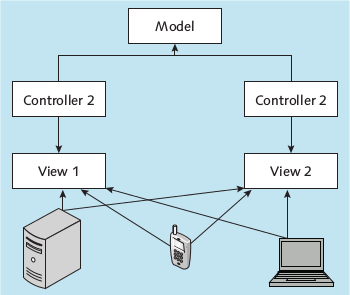
\includegraphics[width=0.5\linewidth]{images/mvc_arch.png}
		\captionof{figure}[Model-View-Controller-Architekturmuster]{Model-View-Controller-Architekturmuster\cite{AntoEinf2014}}
		\label{fig:mvcarch}
	\end{minipage}

\subsubsection{OData Protokoll}
// Einführung in SAPUI5 S. 168 \\
// SAP Netweaver Gateway OData Services\\

\pagebreak
% ----------------------------------------------------------------------------------------------------------
% Kapitel
% ----------------------------------------------------------------------------------------------------------
\section{Fallbeispiel SAP UI5}
Lorem ipsum dolor sit amet.

\subsection{Beschreibung}
// Frontend\\
// Backend\\
// Analyse der wichtigen Arbeitsschritte\\
// Anbindung von \ac{SPP} als Datenquelle ansprechen\\

\subsection{Hilfsmittel}
\subsubsection{Entwicklungsumgebung}
// Kurze Beschreibung der Entwicklungsumgebung\\
// Sprich Eclipse, SE80, Chrome Dev-tools\\
// Neptune Application Designer\\

\subsubsection{UI Design und Prototyping}
// Wireframing als Prototyping\\

\subsubsection{PLATZHALTER}
// HIER KÖNNTE IHRE WERBUNG STEHEN \cite{NilsBlog2014}\\

\subsection{Umsetzung}
\subsubsection{View}
// Auszugsweise Coding bringen um bestimmte Elemente aus der Theorie zu zeigen\\
// Generellen Aufbau der Views erklären\\
// Kapselung wird dadurch verdeutlicht\\
// Listings lassen sich im Text referenzieren: Listing \ref{lst:app.view.js}
	\vspace{1em}
	\begin{lstlisting}[caption=Root View der Applikation, label=lst:app.view.js]
sap.ui.jsview("abat.Mockup.view.App", {

	getControllerName: function () {
		return "abat.Mockup.view.App";
	},
	
	createContent: function (oController) {
		
		// to avoid scroll bars on desktop the root view must be set to block display
		this.setDisplayBlock(true);
		
		// create app
		this.app = new sap.m.SplitApp();

		// load the master page
		var master = sap.ui.xmlview("Master", "abat.Mockup.view.Master");
		master.getController().nav = this.getController();
		this.app.addPage(master, true);
		
		// load the empty page
		var empty = sap.ui.xmlview("Empty", "abat.Mockup.view.Empty");
		this.app.addPage(empty, false);
		
		// wrap app with shell
		return new sap.m.Shell("Shell", {
			title : "{i18n>ShellTitle}",
			showLogout : false,
			app : this.app
		});
	}
});
	\end{lstlisting}

\subsubsection{Model und Controller}
// die Verbindung von beiden Anhand von Coding zeigen\\

\subsubsection{Backend}
// ABAP Stack der den RESTful Service bereitstellt zeigen\\
// Beispielhafte Implementation des HTTP Responses\\

\subsubsection{Analyse}
// Angewandte Analyse mit Heatmap\\
// Mobile First/Responsive Design\\

\pagebreak

% ----------------------------------------------------------------------------------------------------------
% Kapitel
% ----------------------------------------------------------------------------------------------------------
\section{Schluss}
Lorem ipsum dolor sit amet.

\subsection{Zusammenfassung}
// Arbeitsgebiete, Produktions \& Dienstleistungsbereiche\\
// Arbeitsergebnisse\\
// Projektziele, Projektergebnisse, Projekttermine\\
// Mitwirkungszeiträume\\
// Liste aller selbst wahrgenommen Aufgaben und Tätigkeiten\\
// Projektmeilensteine\\
// Ablauforganisation \& Beteiligte\\
// Arbeitsformen, Arbeitsmittel, Arbeitsabläufe\\
// Kommunikations- / Informationsgewohnheiten\\
// Auswertung relevanter Literatur\\
// Themen aus Lehrveranstaltungen\\

\subsection{Bewertung}
// Wesentliche Erkenntnisse und Erfahrungen\\
// Folgerungen und Konsequenzen\\
// Vorschläge für Verbesserung und Veränderung\\
// Auswirkungen auf persönliche Berufs- und Karriereplanung\\
// Bezug zum Studium\\
// hilfreiche Studieninhalte\\
// neu gewonnenes Interesse\\
\pagebreak

%
----------------------------------------------------------------------------------------------------------
% Literatur
% ----------------------------------------------------------------------------------------------------------
\renewcommand\refname{Quellenverzeichnis}
\bibliographystyle{myalpha}
\bibliography{bibo}
\pagebreak

% ----------------------------------------------------------------------------------------------------------
% Anhang
% ----------------------------------------------------------------------------------------------------------
\pagenumbering{Roman}
\setcounter{page}{1}
\lhead{Anhang \thesection}

\begin{appendix}
\section*{Anhang}
\phantomsection
\addcontentsline{toc}{section}{Anhang}
\addtocontents{toc}{\vspace{-0.5em}}

\section{GUI}
Ein toller Anhang.

\subsection*{Screenshot}
\label{app:screenshot}
Unterkategorie, die nicht im Inhaltsverzeichnis auftaucht.

\end{appendix}

\newpage
\thispagestyle{empty}
\begin{center}
	\vspace*{5em}
	\huge\textbf{Erklärung}\\
\end{center}
\vspace{2em}
Hiermit versichere ich, dass ich meine Abschlussarbeit selbständig verfasst und keine anderen als die angegebenen Quellen und Hilfsmittel benutzt habe.

\vspace{4em}
\begin{minipage}{\linewidth}
	\begin{tabular}{p{15em}p{15em}}
		Datum: &  .......................................................\\
		& \centering (Unterschrift)\\
	\end{tabular}
\end{minipage}

\end{document}
